% The cloud-optimized architecture of PR #476: how get_daily and
% get_continuous divide a query into chunks and route each chunk.
% The edge hops are what the response headers showed on 2026-11-23.
\documentclass[tikz,border=8pt]{standalone}
\usepackage[T1]{fontenc}
\usepackage[scaled]{helvet}
\renewcommand{\familydefault}{\sfdefault}
\usetikzlibrary{arrows.meta,backgrounds,calc,fit}

\definecolor{api}{HTML}{1F5FA8}
\definecolor{cat}{HTML}{C2620A}
\definecolor{fil}{HTML}{2E7D32}

\begin{document}
\hyphenpenalty=10000
\exhyphenpenalty=10000
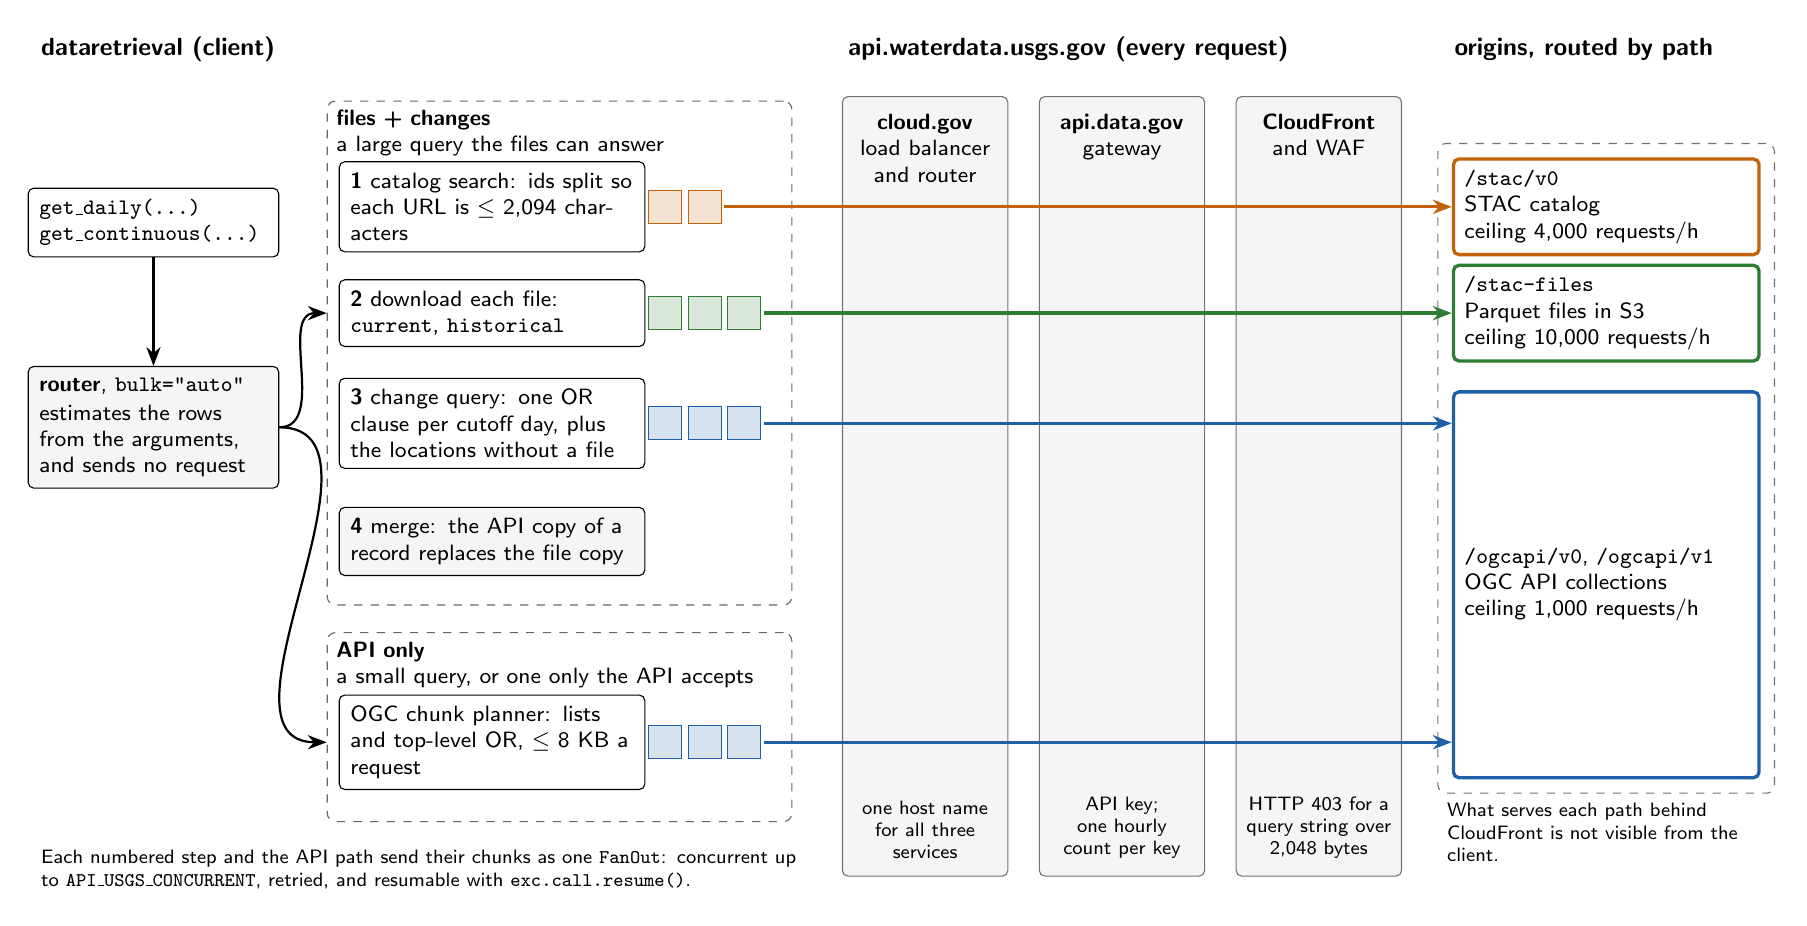
\begin{tikzpicture}[
  font=\sffamily\footnotesize,
  >={Stealth[length=2.4mm]},
  box/.style={draw, rounded corners=2pt, align=left, fill=white,
    inner sep=4pt, text width=#1},
  box/.default=3.6cm,
  tile/.style={draw=#1, fill=#1!18, minimum width=4.2mm,
    minimum height=4.2mm, inner sep=0pt},
  flow/.style={->, very thick, draw=#1},
  hop/.style={draw=black!55, fill=black!4, rounded corners=2pt},
  frame/.style={draw=black!60, dashed, rounded corners=3pt,
    minimum width=5.9cm, anchor=north west},
  frametitle/.style={anchor=north west, align=left, text width=5.6cm},
  title/.style={font=\sffamily\small\bfseries},
]

% ---------------------------------------------------------------- client
\node[title, anchor=west] at (0, 11.1) {dataretrieval (client)};

\node[box=2.9cm] (call) at (1.55, 8.9)
  {\texttt{get\_daily(...)}\\\texttt{get\_continuous(...)}};
\node[box=2.9cm, fill=black!4] (router) at (1.55, 6.3)
  {\textbf{router}, \texttt{bulk="auto"}\\[1pt]
   estimates the rows from the arguments, and sends no request};
\draw[->, thick] (call) -- (router);

% the cloud-optimized path
\node[frame, minimum height=6.4cm] (filesframe) at (3.75, 10.45) {};
\node[frametitle] at (filesframe.north west)
  {\textbf{files + changes}\\a large query the files can answer};

\node[box] (s1) at (5.85, 9.1)
  {\textbf{1} catalog search: ids split so each URL is $\le$ 2,094
   characters};
\node[box] (s2) at (5.85, 7.75)
  {\textbf{2} download each file:\\\texttt{current}, \texttt{historical}};
\node[box] (s3) at (5.85, 6.35)
  {\textbf{3} change query: one OR clause per cutoff day, plus the
   locations without a file};
\node[box, fill=black!4] (s4) at (5.85, 4.85)
  {\textbf{4} merge: the API copy of a record replaces the file copy};

\foreach \i in {0,1} \node[tile=cat] at ($(8.05,9.1)+(\i*0.5,0)$) {};
\foreach \i in {0,1,2} \node[tile=fil] at ($(8.05,7.75)+(\i*0.5,0)$) {};
\foreach \i in {0,1,2} \node[tile=api] at ($(8.05,6.35)+(\i*0.5,0)$) {};

% the API path
\node[frame, minimum height=2.4cm] (apiframe) at (3.75, 3.7) {};
\node[frametitle] at (apiframe.north west)
  {\textbf{API only}\\a small query, or one only the API accepts};
\node[box] (a1) at (5.85, 2.3)
  {OGC chunk planner: lists and top-level OR, $\le$ 8 KB a request};
\foreach \i in {0,1,2} \node[tile=api] at ($(8.05,2.3)+(\i*0.5,0)$) {};

\draw[->, thick] (router.east) to[out=0, in=180] (filesframe.west |- s2);
\draw[->, thick] (router.east) to[out=0, in=180] (apiframe.west |- a1);

\node[align=left, anchor=north west, text width=9.6cm,
  font=\sffamily\scriptsize] at (0, 1.05)
  {Each numbered step and the API path send their chunks as one
   \texttt{FanOut}: concurrent up to \texttt{API\_USGS\_CONCURRENT},
   retried, and resumable with \texttt{exc.call.resume()}.};

% ------------------------------------------------------------------ edge
\node[title, anchor=west] at (10.25, 11.1)
  {api.waterdata.usgs.gov (every request)};

\begin{scope}[on background layer]
  \draw[hop] (10.3, 0.6) rectangle (12.4, 10.5);
  \draw[hop] (12.8, 0.6) rectangle (14.9, 10.5);
  \draw[hop] (15.3, 0.6) rectangle (17.4, 10.5);
\end{scope}
\node[align=center, anchor=north] at (11.35, 10.4)
  {\textbf{cloud.gov}\\load balancer\\and router};
\node[align=center, anchor=north] at (13.85, 10.4)
  {\textbf{api.data.gov}\\gateway};
\node[align=center, anchor=north] at (16.35, 10.4)
  {\textbf{CloudFront}\\and WAF};
\node[align=center, anchor=south, font=\sffamily\scriptsize] at (11.35, 0.7)
  {one host name\\for all three\\services};
\node[align=center, anchor=south, font=\sffamily\scriptsize] at (13.85, 0.7)
  {API key;\\one hourly\\count per key};
\node[align=center, anchor=south, font=\sffamily\scriptsize] at (16.35, 0.7)
  {HTTP 403 for a\\query string over\\2,048 bytes};

% --------------------------------------------------------------- origins
\node[title, anchor=west] at (17.95, 11.1) {origins, routed by path};

\node[box=3.6cm, draw=cat, very thick] (o1) at (20.0, 9.1)
  {\texttt{/stac/v0}\\STAC catalog\\ceiling 4,000 requests/h};
\node[box=3.6cm, draw=fil, very thick] (o2) at (20.0, 7.75)
  {\texttt{/stac-files}\\Parquet files in S3\\ceiling 10,000 requests/h};
\node[box=3.6cm, draw=api, very thick, minimum height=4.9cm] (o3)
  at (20.0, 4.3)
  {\texttt{/ogcapi/v0}, \texttt{/ogcapi/v1}\\OGC API collections\\ceiling
   1,000 requests/h};
\node[draw=black!55, dashed, rounded corners=3pt, fit=(o1)(o3),
  inner sep=5pt] (origins) {};
\node[align=left, anchor=north west, text width=4.1cm,
  font=\sffamily\scriptsize] at (origins.south west)
  {What serves each path behind CloudFront is not visible from the
   client.};

% ----------------------------------------------------------------- flows
\draw[flow=cat] (8.8, 9.1) -- (o1.west);
\draw[flow=fil] (9.3, 7.75) -- (o2.west);
\draw[flow=api] (9.3, 6.35) -- (o3.west |- 0, 6.35);
\draw[flow=api] (9.3, 2.3) -- (o3.west |- 0, 2.3);

\end{tikzpicture}
\end{document}
